	
	\paragraph{QuizziPedia::Front-End::ModelViews::TrainingModelView}
	
	\label{QuizziPedia::Front-End::ModelViews::TrainingModelView}
	
	\begin{figure}[ht]
		\centering
		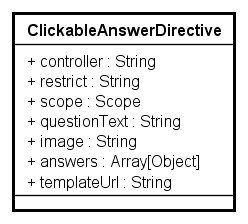
\includegraphics[scale=0.5,keepaspectratio]{UML/Classi/Front-End/QuizziPedia_Front-end_Templates_ClickableAnswerTemplate.png}
		\caption{QuizziPedia::Front-End::ModelViews::LoginModelView}
	\end{figure} \FloatBarrier
	
	\begin{itemize}
		\item \textbf{Descrizione}: classe di tipo modelview la cui istanziazione è contenuta all'interno della variabile di ambiente \$scope di \textit{Angular.js\ped{G}}. All'interno di essa sono presenti le variabili e i metodi necessari per il \textit{Two-Way Data-Binding\ped{G}} tra la view \texttt{TrainingView} e il controller \texttt{TrainingController};
		\item \textbf{Utilizzo}: viene utilizzata per effettuare il \textit{Two-Way Data-Binding\ped{G}} tra la view \texttt{TrainingView} e il controller \texttt{TrainingController} rendendo disponibili variabili e metodi;
		\item \textbf{Relazioni con altre classi}: 
		\begin{itemize}
			\item \textit{OUT} \texttt{TrainingView}: view principale della modalità allenamento, conterrà i vari templates di ogni domanda dell'allenamento; 
			\item \textit{OUT} \texttt{TrainingController}: questa classe permette di gestire la modalità allenamento sottoponendo all'utente le giuste domande adatte al suo livello;
		\end{itemize}
		\item \textbf{Attributi}: 
		\begin{itemize}
			\item \textit{+ topic: String} \\
			Attributo contenente l'argomento scelto dall'utente per l'allenamento;
			\item \textit{+ keywords: Array[String]}\\
			Attributo contenente l'\texttt{array} di keywords scelte dall'utente per l'allenamento;
		\end{itemize}
		\item \textbf{Metodi}: 
		\begin{itemize}
			\item \texttt{+} \texttt{addQuestion(question: QuestionItemModel): void} \\
			Metodo che gestisce l'evento per inserire una domanda nella cronologia delle domande. \\
			\textbf{Parametri}:
			\begin{itemize}
				\item \texttt{question: QuestionItemModel} \\
				Parametro contenente un riferimento all'oggetto di tipo \texttt{QuestionItemModel};
			\end{itemize}
			\item \texttt{+} \texttt{loadNewQuestionBy(topic: String, keywords: Array[String], level: Number): void} \\
			Metodo che emette l'evento per scaricare una nuova domanda in base ai parametri passati. \\
			\textbf{Parametri}:
			\begin{itemize}
				\item \texttt{topic: String} \\
				Parametro contenente l'argomento della domanda;
				\item \texttt{keywords: Array[String]} \\
				Parametro contenente un\texttt{array} di stringhe che rappresenta le keywords scelte per l'allenamento;
				\item \texttt{level: Number} \\
				Parametro contenente il livello dell'utente;
			\end{itemize}
		\end{itemize}
	\end{itemize}
	
	\paragraph{QuizziPedia::Front-End::ModelViews::FillingQuestionnaireModelView}
	
	\label{QuizziPedia::Front-End::ModelViews::FillingQuestionnaireModelView}
	
	\begin{figure}[ht]
		\centering
		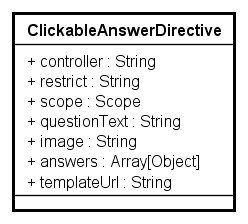
\includegraphics[scale=0.5,keepaspectratio]{UML/Classi/Front-End/QuizziPedia_Front-end_Templates_ClickableAnswerTemplate.png}
		\caption{QuizziPedia::Front-End::ModelViews::SignUpModelView}
	\end{figure} \FloatBarrier
	
	\begin{itemize}
		\item \textbf{Descrizione}: classe di tipo modelview la cui istanziazione è contenuta all'interno della variabile di ambiente \$scope di \textit{Angular.js\ped{G}}. All'interno di essa sono presenti le variabili e i metodi necessari per il \textit{Two-Way Data-Binding\ped{G}} tra la view \texttt{FillingQuestionnaireView} e il controller \texttt{FillingQuestionnaireController};
		\item \textbf{Utilizzo}: viene utilizzata per effettuare il \textit{Two-Way Data-Binding\ped{G}} tra la view \texttt{FillingQuestionnaireView} e il controller \texttt{FillingQuestionnaireController} rendendo disponibili variabili e metodi;
		\item \textbf{Relazioni con altre classi}: 
		\begin{itemize}
			\item \textit{OUT} \texttt{FillingQuestionnaireView}: view principale per la compilazione del questionario. Conterrà i vari templates di ogni domanda appartenente al questionario; 
			\item \textit{OUT} \texttt{FillingQuestionnaireController}: questa classe permette di gestire la compilazione del questionario;
		\end{itemize}
		\item \textbf{Attributi}: 
		\begin{itemize}
			\item \texttt{+ title: String}\\
			Questo attributo rappresenta il titolo del questionario;
			\item \texttt{+ author: ObjectId}\\
			Questo attributo rappresenta l'autore del questionario;
	
		\end{itemize}
		\item \textbf{Metodi}: 
		\begin{itemize}
			\item \texttt{+} \texttt{loadNextQuestion(question: QuestionItemModel): void}: \\ Metodo che invoca l'evento per visualizzare la domanda successiva del quiz tramite QuestionController; \\
			\textbf{Parametri}:
			\begin{itemize}
				\item \texttt{question: QuestionItemModel} \\
				Parametro contenente un riferimento all'oggetto di tipo \texttt{QuestionItemModel}.
			\end{itemize}
			\item \texttt{+} \texttt{loadPreviousQuestion(question: QuestionItemModel): void}: \\ Metodo che invoca l'evento per visualizzare la domanda precedente del quiz tramite QuestionController; \\
			\textbf{Parametri}:
			\begin{itemize}
				\item \texttt{question: QuestionItemModel} \\
				Parametro contenente un riferimento all'oggetto di tipo \texttt{QuestionItemModel}.
			\end{itemize}
		\end{itemize}
	\end{itemize}
	
	\paragraph{QuizziPedia::Front-End::ModelViews::CreateQuestionnaireModelView}
	
	\label{QuizziPedia::Front-End::ModelViews::CreateQuestionnaireModelView}
	
	\begin{figure}[ht]
		\centering
		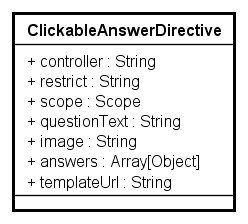
\includegraphics[scale=0.5,keepaspectratio]{UML/Classi/Front-End/QuizziPedia_Front-end_Templates_ClickableAnswerTemplate.png}
		\caption{QuizziPedia::Front-End::ModelViews::PasswordForgotModelView}
	\end{figure} \FloatBarrier
	
	\begin{itemize}
		\item \textbf{Descrizione}: classe di tipo modelview la cui istanziazione è contenuta all'interno della variabile di ambiente \$scope di \textit{Angular.js\ped{G}}. All'interno di essa sono presenti le variabili e i metodi necessari per il \textit{Two-Way Data-Binding\ped{G}} tra la view \texttt{CreateQuestionnaireView} e il controller \texttt{CreateQuestionnaireController};
		\item \textbf{Utilizzo}: viene utilizzata per effettuare il \textit{Two-Way Data-Binding\ped{G}} tra la view \texttt{CreateQuestionnaireView} e il controller \texttt{CreateQuestionnaireController} rendendo disponibili variabili e metodi;
		\item \textbf{Relazioni con altre classi}: 
		\begin{itemize}
			\item \textit{OUT} \texttt{CreateQuestionnaireView}: view per la creazione del questionario; 
			\item \textit{OUT} \texttt{CreateQuestionnaireController}: questa classe permette di gestire la creazione di un questionario;
		\end{itemize}
		\item \textbf{Attributi}: 
		\begin{itemize}
			\item \texttt{+ nameQuestionnaire: String}: \\ Attributo che specifica il nome del questionario creato;
			\item \texttt{+ topics: Array} \\ Array contenente le stringhe dei nomi degli argomenti;
			\item \texttt{+ keyword: String} \\ Attributo contenente la keyword associata alla domanda/questionario;
			\item \texttt{+ question: String} \\ Attributo che conterrà la stringa per la ricerca della domanda;
			\item \texttt{+ questions: Array} \\ Array contenente le domande trovate durante la ricerca;
			\item \texttt{+ questionsChosen: Array} \\ Array contenente le domande inserite nel questionario;
		\end{itemize}
		\item \textbf{Metodi}: 
		\begin{itemize}
			\item \texttt{+} \texttt{createQuestionnaire(title: String, quiz: QuestionnaireModel)}: \\Metodo che permette di inserire un questionario nel database tramite richiesta al service; \\
			\textbf{Parametri}:
			\begin{itemize}
				\item 
			\end{itemize}
			\item \texttt{+} \texttt{modifyQuestionnaire(quizId: QuestionnaireModel)}: \\ Metodo che serve per modificare un questionario; \\
			\textbf{Parametri}:
			\begin{itemize}
				\item \texttt{quiz: QuestionnaireModel}: parametro che rappresenta l'oggetto questionario;
			\end{itemize}
			\item \texttt{+} \texttt{getQuestionnaire(quizId: String)}: \\Metodo che serve per ottenere un questionario tramite l'id in modo da poterlo modificare; \\
			\textbf{Parametri}:
			\begin{itemize}
				\item \texttt{quizId: String}: parametro che rappresenta l'id del questionario da richiedere.
			\end{itemize}
			\item \texttt{+} \texttt{getQuestionnairePreview(username: String)}: \\ Metodo che serve per ottenere la lista di tutti i questionari di un utente; \\
			\textbf{Parametri}:
			\begin{itemize}
				\item \texttt{username: String}: parametro che indica l'utente del quale vogliamo caricare tutti i questionari.
			\end{itemize}
			\item \texttt{+} \texttt{deleteQuestionnaire(quizId: String): void}: \\Metodo che elimina un questionario.
			\textbf{Parametri}:
			\texttt{quizId: String}: identificativo del questionario da eliminare.
		\end{itemize}
	\end{itemize}
	
	\paragraph{QuizziPedia::Front-End::ModelViews::RegistrationManagementModelView}
	
	\label{QuizziPedia::Front-End::ModelViews::RegistrationManagementModelView}
	
	\begin{figure}[ht]
		\centering
		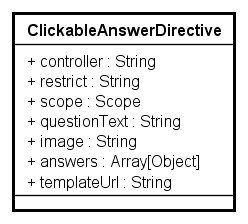
\includegraphics[scale=0.5,keepaspectratio]{UML/Classi/Front-End/QuizziPedia_Front-end_Templates_ClickableAnswerTemplate.png}
		\caption{QuizziPedia::Front-End::ModelViews::HomeModelView}
	\end{figure} \FloatBarrier
	
	\begin{itemize}
		\item \textbf{Descrizione}: classe di tipo modelview la cui istanziazione è contenuta all'interno della variabile di ambiente \$scope di \textit{Angular.js\ped{G}}. All'interno di essa sono presenti le variabili e i metodi necessari per il \textit{Two-Way Data-Binding\ped{G}} tra la view \texttt{RegistrationManagementView} e il controller \texttt{RegistrationManagementController};
		\item \textbf{Utilizzo}: viene utilizzata per effettuare il \textit{Two-Way Data-Binding\ped{G}} tra la view \texttt{RegistrationManagementView} e il controller \texttt{RegistrationManagementController} rendendo disponibili variabili e metodi;
		\item \textbf{Relazioni con altre classi}: 
		\begin{itemize}
			\item \textit{IN} \texttt{RegistrationManagementView}: view per la gestione degli utenti iscritti a un proprio questionario; 
			\item \textit{IN} \texttt{RegistrationManagementController}: questa classe permette di gestire le iscrizione degli utenti ai questionari;
		\end{itemize}
		\item \textbf{Attributi}: 
		\begin{itemize}
			\item \texttt{+ subscribers: Array} \\ Array contenete un oggetto per ogni utente iscritto al questionario. L'oggetto sarà composto dai campi \texttt{nome} e \texttt{cognome};
		\end{itemize}
		\item \textbf{Metodi}: 
		\begin{itemize}
			\item \texttt{subscribeQuestionnaire(username: String): void} \\ Metodo che permette l'iscrizione ad un questionario. Richiama la funzionalità del QuizService. \\
			\textbf{Parametri}:
			\begin{itemize}
				\item \texttt{username: String}: parametro che indica l'utente da iscrivere al questionario.
			\end{itemize}
		\end{itemize}
	\end{itemize}
	
	\paragraph{QuizziPedia::Front-End::ModelViews::ResultsOfQuizzesModelView}
	
	\label{QuizziPedia::Front-End::ModelViews::ResultsOfQuizzesModelView}
	
	\begin{figure}[ht]
		\centering
		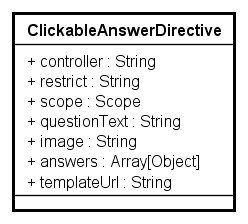
\includegraphics[scale=0.5,keepaspectratio]{UML/Classi/Front-End/QuizziPedia_Front-end_Templates_ClickableAnswerTemplate.png}
		\caption{QuizziPedia::Front-End::ModelViews::HomeModelView}
	\end{figure} \FloatBarrier
	
	\begin{itemize}
		\item \textbf{Descrizione}: classe di tipo modelview la cui istanziazione è contenuta all'interno della variabile di ambiente \$scope di \textit{Angular.js\ped{G}}. All'interno di essa sono presenti le variabili e i metodi necessari per il \textit{Two-Way Data-Binding\ped{G}} tra la view \texttt{ResultsView} e il controller \texttt{ResultsController};
		\item \textbf{Utilizzo}: viene utilizzata per effettuare il \textit{Two-Way Data-Binding\ped{G}} tra la view \texttt{ResultsView} e il controller \texttt{ResultsController} rendendo disponibili variabili e metodi;
		\item \textbf{Relazioni con altre classi}: 
		\begin{itemize}
			\item \textit{IN} \texttt{ResultsView}: view contenente i risultati della ricerca effettuata, sia gli utenti che i questionari trovati; 
			\item \textit{IN} \texttt{ResultsController}: questa classe permette di gestire le iscrizione degli utenti ai questionari;
		\end{itemize}
		\item \textbf{Attributi}: 
		\begin{itemize}
			\item ;
		\end{itemize}
		\item \textbf{Metodi}: 
		\begin{itemize}
			\item ;
		\end{itemize}
	\end{itemize}
	
	\paragraph{QuizziPedia::Front-End::ModelViews::QuestionnaireManagementModelView}
	
	\label{QuizziPedia::Front-End::ModelViews::QuestionnaireManagementModelView}
	
	\begin{figure}[ht]
		\centering
		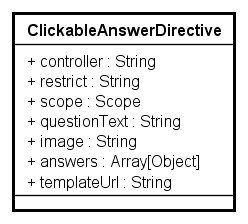
\includegraphics[scale=0.5,keepaspectratio]{UML/Classi/Front-End/QuizziPedia_Front-end_Templates_ClickableAnswerTemplate.png}
		\caption{QuizziPedia::Front-End::ModelViews::QuestionnaireManagementModelView}
	\end{figure} \FloatBarrier
	
	\begin{itemize}
		\item \textbf{Descrizione}: classe di tipo modelview la cui istanziazione è contenuta all'interno della variabile di ambiente \$scope di \textit{Angular.js\ped{G}}. All'interno di essa sono presenti le variabili e i metodi necessari per il \textit{Two-Way Data-Binding\ped{G}} tra la view \texttt{QuestionnaireManagementView} e il controller \texttt{QuestionnaireManagementController};
		\item \textbf{Utilizzo}: viene utilizzata per effettuare il \textit{Two-Way Data-Binding\ped{G}} tra la view \texttt{QuestionnaireManagementView} e il controller \texttt{QuestionnaireManagementController} rendendo disponibili variabili e metodi;
		\item \textbf{Relazioni con altre classi}: 
		\begin{itemize}
			\item \textit{IN} \texttt{QuestionnaireManagementView}: view principale per la gestione dei questionari; 
			\item \textit{IN} \texttt{QuestionnaireManagementController}: questa classe permette di gestire tutti i questionari creati da un utente;
		\end{itemize}
		\item \textbf{Attributi}: 
		\begin{itemize}
			\item ;
		\end{itemize}
		\item \textbf{Metodi}: 
		\begin{itemize}
			\item ;
		\end{itemize}
	\end{itemize}
	
	\paragraph{QuizziPedia::Front-End::ModelViews::QuestionnaireDetailsModelView}
	
	\label{QuizziPedia::Front-End::ModelViews::QuestionnaireDetailsModelView}
	
	\begin{figure}[ht]
		\centering
		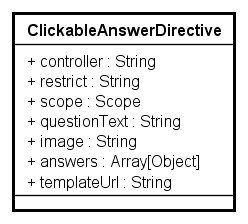
\includegraphics[scale=0.5,keepaspectratio]{UML/Classi/Front-End/QuizziPedia_Front-end_Templates_ClickableAnswerTemplate.png}
		\caption{QuizziPedia::Front-End::ModelViews::QuestionnaireDetailsModelView}
	\end{figure} \FloatBarrier
	
	\begin{itemize}
		\item \textbf{Descrizione}: classe di tipo modelview la cui istanziazione è contenuta all'interno della variabile di ambiente \$scope di \textit{Angular.js\ped{G}}. All'interno di essa sono presenti le variabili e i metodi necessari per il \textit{Two-Way Data-Binding\ped{G}} tra la view \texttt{UserView} e il controller \texttt{QuestionnaireDetailsController};
		\item \textbf{Utilizzo}: viene utilizzata per effettuare il \textit{Two-Way Data-Binding\ped{G}} tra la view \texttt{UserView} e il controller \texttt{QuestionnaireDetailsController} rendendo disponibili variabili e metodi;
		\item \textbf{Relazioni con altre classi}: 
		\begin{itemize}
			\item \textit{IN} \texttt{UserView}: view contenente le direttive dei dati personali dell'utente, delle sue statistiche relative ai questionari e agli allenamenti effettuati e dei questionari a cui è iscritto; 
			\item \textit{IN} \texttt{QuestionnaireDetailsController}: questa classe permette di gestire i dettagli di un questionario;
		\end{itemize}
		\item \textbf{Attributi}: 
		\begin{itemize}
			\item ;
		\end{itemize}
		\item \textbf{Metodi}: 
		\begin{itemize}
			\item ;
		\end{itemize}
	\end{itemize}
	
		\paragraph{QuizziPedia::Front-End::ModelViews::UserDetailsModelView}
		
		\label{QuizziPedia::Front-End::ModelViews::UserDetailsModelView}
		
		\begin{figure}[ht]
			\centering
			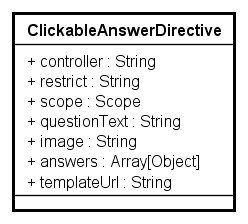
\includegraphics[scale=0.5,keepaspectratio]{UML/Classi/Front-End/QuizziPedia_Front-end_Templates_ClickableAnswerTemplate.png}
			\caption{QuizziPedia::Front-End::ModelViews::UserDetailsModelView}
		\end{figure} \FloatBarrier
		
		\begin{itemize}
			\item \textbf{Descrizione}: classe di tipo modelview la cui istanziazione è contenuta all'interno della variabile di ambiente \$scope di \textit{Angular.js\ped{G}}. All'interno di essa sono presenti le variabili e i metodi necessari per il \textit{Two-Way Data-Binding\ped{G}} tra la view \texttt{UserView} e il controller \texttt{UserDetailsController};
			\item \textbf{Utilizzo}: viene utilizzata per effettuare il \textit{Two-Way Data-Binding\ped{G}} tra la view \texttt{UserView} e il controller \texttt{UserDetailsController} rendendo disponibili variabili e metodi;
			\item \textbf{Relazioni con altre classi}: 
			\begin{itemize}
				\item \textit{IN} \texttt{UserView}: view contenente le direttive dei dati personali dell'utente, delle sue statistiche relative ai questionari e agli allenamenti effettuati e dei questionari a cui è iscritto; 
				\item \textit{IN} \texttt{UserDetailsController}: questa classe permette di ottenere i dati di un utente;
			\end{itemize}
			\item \textbf{Attributi}: 
			\begin{itemize}
				\item ;
			\end{itemize}
			\item \textbf{Metodi}: 
			\begin{itemize}
				\item ;
			\end{itemize}
		\end{itemize}
		
			\paragraph{QuizziPedia::Front-End::ModelViews::QuestionsModelView}
			
			\label{QuizziPedia::Front-End::ModelViews::QuestionsModelView}
			
			\begin{figure}[ht]
				\centering
				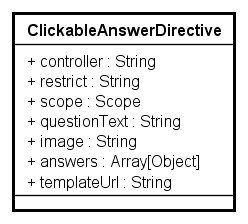
\includegraphics[scale=0.5,keepaspectratio]{UML/Classi/Front-End/QuizziPedia_Front-end_Templates_ClickableAnswerTemplate.png}
				\caption{QuizziPedia::Front-End::ModelViews::QuestionsModelView}
			\end{figure} \FloatBarrier
			
			\begin{itemize}
				\item \textbf{Descrizione}: classe di tipo modelview la cui istanziazione è contenuta all'interno della variabile di ambiente \$scope di \textit{Angular.js\ped{G}}. All'interno di essa sono presenti le variabili e i metodi necessari per il \textit{Two-Way Data-Binding\ped{G}} tra le directive che compongono dinamicamente la vista della domanda e il controller \texttt{QuestionsController};
				\item \textbf{Utilizzo}: viene utilizzata per effettuare il \textit{Two-Way Data-Binding\ped{G}} tra le directive che compongono dinamicamente la vista della domanda e il controller \texttt{QuestionsController} rendendo disponibili variabili e metodi;
				\item \textbf{Relazioni con altre classi}: 
				\begin{itemize} 
					\item \textit{OUT} \texttt{QuestionsController}: questa classe permette di gestire il recupero delle domande per poterle stampare nella modalità allenamento;
					\item \textit{OUT} \texttt{ClickableAnswerDirective}: rappresenta il componente grafico che permette all'utente di visualizzare la domanda ad area cliccabile nell'immagine. Viene visualizzato dinamicamente all'interno delle views TrainingView e FillingQuestionnaireView mediante il controller QuestionsController;
					\item \textit{OUT} \texttt{EmptySpaceAnswerDirective}: rappresenta il componente grafico che permette all'utente di visualizzare l'esercizio a riempimento di spazi vuoti. Viene visualizzato dinamicamente all'interno delle views TrainingView e FillingQuestionnaireView mediante il controller QuestionsController;
					\item \textit{OUT} \texttt{HeaderTextQuestionDirective}: rappresenta il componente grafico che presenta all'utente il testo della domanda, l'argomento e le parole chiave. Viene visualizzato dinamicamente all'interno delle views TrainingView e FillingQuestionnaireView mediante il controller QuestionsController;
					\item \textit{OUT} \texttt{LinkingAnswerDirective}: rappresenta il componente grafico che permette all'utente di visualizzare la domanda di collegamento. Viene visualizzato dinamicamente all'interno delle views TrainingView e FillingQuestionnaireView mediante il controller QuestionsController;
					\item \textit{OUT} \texttt{MultipleChoiceAnswerDirective}: rappresenta il componente grafico che permette all'utente di visualizzare la domanda a risposta multipla. Viene visualizzato dinamicamente all'interno delle views TrainingView e FillingQuestionnaireView mediante il controller QuestionsController;
					\item \textit{OUT} \texttt{SortImagesAnswerDirective}: rappresenta il componente grafico che permette all'utente di visualizzare la domanda ad ordinamento di immagini. Viene visualizzato dinamicamente all'interno delle views TrainingView e FillingQuestionnaireView mediante il controller QuestionsController;
					\item \textit{OUT} \texttt{SortTextAnswerDirective}: rappresenta il componente grafico che permette all'utente di visualizzare la domanda ad ordinamento di stringhe. Viene visualizzato dinamicamente all'interno delle views TrainingView e FillingQuestionnaireView mediante il controller QuestionsController;
					\item \textit{OUT} \texttt{TrainingSetUpDirective}: rappresenta il componente grafico che permette all'utente di selezionare l'argomento e le parole chiave per iniziare un allenamento con queste caratteristiche. Viene visualizzato dinamicamente all'interno della view TrainingView mediante il controller TrainingController;
					\item \textit{OUT} \texttt{TrueFalseAnswareDirective}: rappresenta il componente grafico che permette all'utente di visualizzare la domanda vero e falso. Viene visualizzato dinamicamente all'interno delle views TrainingView e FillingQuestionnaireView mediante il controller QuestionsController;					
				\end{itemize}
				\item \textbf{Attributi}: 
				\begin{itemize}
					\item \texttt{+ piecesOfQuestion: Array[Object]} \\
					Questo attributo è un \texttt{array} di \texttt{Object} contenente la domanda da visualizzare dinamicamente attraverso le direttive all'interno le direttive di allenamento e di compilazione dei questionari;
					\item \texttt{+ objAnswer: Array[Object]} \\
					Questo attributo è un \texttt{array} di \texttt{Object} contenente le risposte date fino a quel momento dall'utente in una domanda. L'\texttt{Object} è così formato: \\
					\begin{itemize}
						\item \texttt{+ typeQuestion: String} \\
						Questo attributo rappresenta il tipo della domanda;
						\item \texttt{+ answerGiven: Array[String]} \\
						Questo attributo rappresenta le riposte scelta dall'utente fino a quel momento.
					\end{itemize}
				\end{itemize}
				\item \textbf{Metodi}: 
				\begin{itemize}
					\item \texttt{+} \texttt{addAnswer(index: Number, typeQuestion: String, answerGiven: Array[String]): void} \\
					Metodo che gestisce l'evento di selezione delle risposte. \\
					\textbf{Parametri}:
					\begin{itemize}
						\item \texttt{index: Number} \\
						Parametro contenente l'indice della risposta di cui si vuole tenere traccia. Rappresenta anche l'indice dell'\texttt{array objAswer} in cui verrà inserito l'oggetto delle risposte date;
						\item \texttt{typeQuestion: String} \\
						Parametro contenente una stringa la quale indica la tipologia della domanda;
						\item \texttt{answerGiven: Array[String]} \\
						Parametro contenente l'array di risposte date dall'utente aggiornato all'ultima iterazione;
					\end{itemize};
					\item \texttt{+} \texttt{answerGiven(index: Number): Array[String]} \\
					Metodo di supporto che ritorna un \texttt{array} di stringhe contenente le risposte date. Si occupa di recuperare le risposte date nelle domande vero/falso, risposta multipla e ad area cliccabile.\\
					\textbf{Parametri}:
					\begin{itemize}
						\item \texttt{index: Number} \\
						Parametro contenente l'indice della risposta di cui si vuole raccogliere le risposte date; 
					\end{itemize}
					\item \texttt{+} \texttt{orderChosen(index: Number): Array[String]} \\
					Metodo di supporto che ritorna un \texttt{array} di stringhe contenente le risposte date. Si occupa di recuperare le risposte date nelle domande ad ordinamento e di riempimento di spazi.\\
					\textbf{Parametri}:
					\begin{itemize}
						\item \texttt{index: Number} \\
						Parametro contenente l'indice della risposta di cui si vuole raccogliere le risposte date; 
					\end{itemize}
					\item \texttt{+} \texttt{linkingMade(index: Number): Array[String]} \\
					Metodo di supporto che ritorna un \texttt{array} di stringhe contenente le risposte date. Si occupa di recuperare le risposte date nelle domande a collegamento.\\
					\textbf{Parametri}:
					\begin{itemize}
						\item \texttt{index: Number} \\
						Parametro contenente l'indice della risposta di cui si vuole raccogliere le risposte date; 
					\end{itemize}
					\item \texttt{+} \texttt{loadNewQuestionBy(topic: String, keywords: Array[String], level: Number): void} \\
					Metodo che gestisce l'evento per scaricare una nuova domanda in base ai parametri passati. \\
					\textbf{Parametri}:
					\begin{itemize}
						\item \texttt{topic: String} \\
						Parametro contenente l'argomento della domanda;
						\item \texttt{keywords: Array[String]} \\
						Parametro contenente un\texttt{array} di stringhe che rappresenta le keywords scelte per l'allenamento;
						\item \texttt{level: Number} \\
						Parametro contenente il livello dell'utente;
					\end{itemize}
					\item \texttt{+} \texttt{loadNewQuestion(question: QuestionItemModel): void} \\
					Metodo che gestisce l'evento per visualizzare una nuova domanda. \\
					\textbf{Parametri}:
					\begin{itemize}
						\item \texttt{question: QuestionItemModel} \\
						Parametro contenente un riferimento all'oggetto di tipo \texttt{QuestionItemModel};
					\end{itemize}
					\item \texttt{+} \texttt{checkAnswer(): boolean} \\ 
					Metodo che controlla che le risposte date siano corrette;
				\end{itemize}
			\end{itemize}
			
				\paragraph{QuizziPedia::Front-End::ModelViews::KeywordsModelView}
				
				\label{QuizziPedia::Front-End::ModelViews::TopicKeywordsModelView}
				
				\begin{figure}[ht]
					\centering
					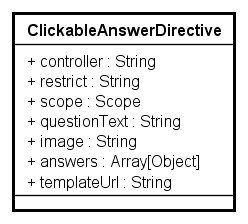
\includegraphics[scale=0.5,keepaspectratio]{UML/Classi/Front-End/QuizziPedia_Front-end_Templates_ClickableAnswerTemplate.png}
					\caption{QuizziPedia::Front-End::ModelViews::TopicKeywordsModelView}
				\end{figure} \FloatBarrier
				
				\begin{itemize}
					\item \textbf{Descrizione}: classe di tipo modelview la cui istanziazione è contenuta all'interno della variabile di ambiente \$scope di \textit{Angular.js\ped{G}}. All'interno di essa sono presenti le variabili e i metodi necessari per il \textit{Two-Way Data-Binding\ped{G}} tra la view \texttt{CreateQuestionnaireView} e il controller \texttt{KeywordsController};
					\item \textbf{Utilizzo}: viene utilizzata per effettuare il \textit{Two-Way Data-Binding\ped{G}} tra la view \texttt{CreateQuestionnaireView} e il controller \texttt{KeywordsController} rendendo disponibili variabili e metodi;
					\item \textbf{Relazioni con altre classi}: 
					\begin{itemize}
						\item \textit{IN} \texttt{CreateQuestionnaireView}: view per la creazione del questionario; 
						\item \textit{IN} \texttt{KeywordsController}: questa classe permette di gestire il recupero delle parole chiave di un questionario;
					\end{itemize}
					\item \textbf{Attributi}: 
					\begin{itemize}
						\item ;
					\end{itemize}
					\item \textbf{Metodi}: 
					\begin{itemize}
						\item ;
					\end{itemize}
				\end{itemize}
				
					\paragraph{QuizziPedia::Front-End::ModelViews::QuestionnaireQuestionsManagementModelView}
					
					\label{QuizziPedia::Front-End::ModelViews::QuestionnaireQuestionsManagementModelView}
					
					\begin{figure}[ht]
						\centering
						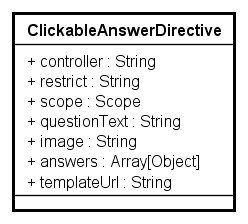
\includegraphics[scale=0.5,keepaspectratio]{UML/Classi/Front-End/QuizziPedia_Front-end_Templates_ClickableAnswerTemplate.png}
						\caption{QuizziPedia::Front-End::ModelViews::QuestionnaireQuestionsManagementModelView}
					\end{figure} \FloatBarrier
					
					\begin{itemize}
						\item \textbf{Descrizione}: classe di tipo modelview la cui istanziazione è contenuta all'interno della variabile di ambiente \$scope di \textit{Angular.js\ped{G}}. All'interno di essa sono presenti le variabili e i metodi necessari per il \textit{Two-Way Data-Binding\ped{G}} tra la view \texttt{QuestionnaireQuestionsManagementView} e il controller \texttt{QuestionnaireQuestionsManagementController};
						\item \textbf{Utilizzo}: viene utilizzata per effettuare il \textit{Two-Way Data-Binding\ped{G}} tra la view \texttt{QuestionnaireQuestionsManagementView} e il controller \texttt{QuestionnaireQuestionsManagementController} rendendo disponibili variabili e metodi;
						\item \textbf{Relazioni con altre classi}: 
						\begin{itemize}
							\item \textit{IN} \texttt{CreateQuestionnaireView}: view per la creazione del questionario; 
							\item \textit{IN} \texttt{QuestionnaireQuestionsManagementController}: questa classe permette di gestire il recupero delle parole chiave di un questionario;
						\end{itemize}
						\item \textbf{Attributi}: 
						\begin{itemize}
							\item ;
						\end{itemize}
						\item \textbf{Metodi}: 
						\begin{itemize}
							\item ;
						\end{itemize}
					\end{itemize}
					
						
							\paragraph{QuizziPedia::Front-End::ModelViews::QuizEventModelView}
							
							\label{QuizziPedia::Front-End::ModelViews::QuizEventModelView}
							
							\begin{figure}[ht]
								\centering
								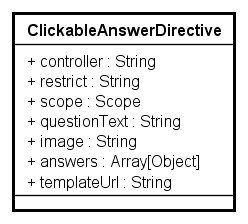
\includegraphics[scale=0.5,keepaspectratio]{UML/Classi/Front-End/QuizziPedia_Front-end_Templates_ClickableAnswerTemplate.png}
								\caption{QuizziPedia::Front-End::ModelViews::QuizEventModelView}
							\end{figure} \FloatBarrier
							
							\begin{itemize}
								\item \textbf{Descrizione}: classe di tipo modelview la cui istanziazione è contenuta all'interno della variabile di ambiente \$scope di \textit{Angular.js\ped{G}}. All'interno di essa sono presenti le variabili e i metodi necessari per il \textit{Two-Way Data-Binding\ped{G}} tra la view \texttt{QuizEventView} e il controller \texttt{QuizEventController};
								\item \textbf{Utilizzo}: viene utilizzata per effettuare il \textit{Two-Way Data-Binding\ped{G}} tra la view \texttt{QuizEventView} e il controller \texttt{QuizEventController} rendendo disponibili variabili e metodi;
								\item \textbf{Relazioni con altre classi}: 
								\begin{itemize}
									\item \textit{IN} \texttt{QuestionnaireManagementView}: view principale per la gestione dei questionari; 
									\item \textit{IN} \texttt{QuizEventController}: questa classe permette di reagire ai comandi dell'utente durante la gestione dei suoi questionari;
								\end{itemize}
								\item \textbf{Attributi}: 
								\begin{itemize}
									\item ;
								\end{itemize}
								\item \textbf{Metodi}: 
								\begin{itemize}
									\item \texttt{+} \texttt{modifyQuestionnaire(quizId: String): void} \\
									Metodo che gestisce l’evento click sul pulsante di modifica questionario. Effettua il redirect alla pagina di gestione questionari;
									\begin{itemize}
										\item \texttt{quizId: String}: parametro che indica l'identificativo univoco di un questionario.
									\end{itemize}
									\item \texttt{+} \texttt{deleteQuestionnaire(quizId: String): void} \\
									Metodo che gestisce l’evento click sul pulsante di eliminazione questionario. Effettua il redirect alla pagina di gestione questionari;  
									\begin{itemize}
										\item \texttt{quizId: String}: parametro che indica l'identificativo univoco di un questionario.
									\end{itemize}
									\item \texttt{+} \texttt{subscribeManagement(quizId: String): void} \\
									Metodo che gestisce l’evento click sul pulsante di gestione iscrizioni. Effettua il redirect alla pagina di gestione iscrizioni;
									\item \texttt{+} \texttt{examModalityquizId: String(): void} \\
									\begin{itemize}
										\item \texttt{quizId: String}: parametro che indica l'identificativo univoco di un questionario.
									\end{itemize}
									Metodo che gestisce l’evento click sul pulsante di attivazione modalità esame. Effettua il redirect alla pagina di gestione questionari;
									\begin{itemize}
										\item \texttt{quizId: String}: parametro che indica l'identificativo univoco di un questionario.
									\end{itemize}
									\item \texttt{+} \texttt{resultsQuestionnaire(quizId: String): void} \\
									Metodo che gestisce l’evento click sul pulsante di allenamento. Effettua il redirect alla pagina di gestine questionari;
									\begin{itemize}
										\item \texttt{quizId: String}: parametro che indica l'identificativo univoco di un questionario.
									\end{itemize}   
								\end{itemize}
							\end{itemize}	
